\documentclass[handout]{beamer}

\usepackage[utf8x]{inputenc}
\usepackage[brazil,british]{babel}
\usetheme{default} 
\usecolortheme{beaver}
\setbeamertemplate{footline}[frame number]
\usepackage{graphicx}
\usepackage{clrscode}
\usepackage{hyperref}
\usepackage{pgf}

% \usecolortheme{dove}
\title{Aula 02: Análise de algoritmos --- arcabouço teórico}
\author{David Déharbe \\
  Programa de Pós-graduação em Sistemas e Computação \\
  Universidade Federal do Rio Grande do Norte \\
  Centro de Ciências Exatas e da Terra \\
  Departamento de Informática e Matemáica Aplicada}
\date{11 de fevereiro de 2015}
\logo{
\includegraphics[width=1cm]{img/logo-ppgsc-icon-text.png}}

\newcommand{\sel}[1]{\textcolor{teal}{#1}}

\begin{document}
\selectlanguage{brazil}
\begin{frame}
  \titlepage
\end{frame}

\begin{frame}
  \frametitle{Plano da aula}
  \tableofcontents
\end{frame}

\section{Introdução}

\begin{frame}

  \frametitle{Contexto}

  \begin{center}
  \begin{pgfpicture}{0cm}{0cm}{9cm}{7.3cm}
  \pgfsetendarrow{\pgfarrowtriangle{3pt}}

  \pgfrect[stroke]{\pgfxy(2,6.5)}{\pgfxy(5,.8)}
  \pgfputat{\pgfxy(4.5,6.9)}{\pgfbox[center,center]{Entender problema}}
  \pgfline{\pgfxy(4.5,6.5)}{\pgfxy(4.5,6.0)}

  \pgfrect[stroke]{\pgfxy(2,5.2)}{\pgfxy(5,.8)}
  \pgfputat{\pgfxy(4.5,5.6)}{\pgfbox[center,center]{Escolher abordagem}}
  \pgfline{\pgfxy(4.5,5.2)}{\pgfxy(4.5,4.7)}

  \pgfrect[stroke]{\pgfxy(2,3.9)}{\pgfxy(5,.8)}
  \pgfputat{\pgfxy(4.5,4.3)}{\pgfbox[center,center]{Projetar algoritmo}}
  \pgfline{\pgfxy(4.5,3.9)}{\pgfxy(4.5,3.4)}

  \pgfrect[stroke]{\pgfxy(2,2.6)}{\pgfxy(5,.8)}
  \pgfputat{\pgfxy(4.5,3.0)}{\pgfbox[center,center]{Provar correção}}
  \pgfline{\pgfxy(4.5,2.6)}{\pgfxy(4.5,2.1)}
  \pgfmoveto{\pgfxy(2.0,3.0)}
  \pgfcurveto{\pgfxy(1.5,3.0)}{\pgfxy(1.5,4.3)}{\pgfxy(2.0,4.3)}
  \pgfstroke
  \pgfmoveto{\pgfxy(2.0,3.0)}
  \pgfcurveto{\pgfxy(1.0,3.0)}{\pgfxy(1.0,5.6)}{\pgfxy(2.0,5.6)}
  \pgfstroke

  \pgfsetcolor{lightgray}
  \pgfrect[fill]{\pgfxy(2,1.3)}{\pgfxy(5,.8)}
  \pgfsetcolor{black}
  \pgfputat{\pgfxy(4.5,1.7)}{\pgfbox[center,center]{Analizar complexidade}}
  \pgfline{\pgfxy(4.5,1.3)}{\pgfxy(4.5,0.8)}
  \pgfmoveto{\pgfxy(7.0,1.7)}
  \pgfcurveto{\pgfxy(7.5,1.7)}{\pgfxy(7.5,4.3)}{\pgfxy(7.0,4.3)}
  \pgfstroke
  \pgfmoveto{\pgfxy(7.0,1.7)}
  \pgfcurveto{\pgfxy(8.0,1.7)}{\pgfxy(8.0,5.6)}{\pgfxy(7.0,5.6)}
  \pgfstroke

  \pgfrect[stroke]{\pgfxy(2,0)}{\pgfxy(5,.8)}
  \pgfputat{\pgfxy(4.5,0.4)}{\pgfbox[center,center]{Codificar algoritmo}}
\end{pgfpicture}
  \end{center}
\end{frame}

\begin{frame}

  \frametitle{Análise de algoritmos}

  \selectlanguage{british}
  \begin{quote}

    analysis

    detailed examination of the elements or structure of something, typically as
    a basis for discussion or interpretation: statistical analysis | an analysis
    of popular culture.

    --- Dictionary Apple 2.2.3
  \end{quote}
  \pause
  \selectlanguage{brazil}
  \begin{itemize}
  \item correção
  \item simplicidade
  \item generalidade
  \item recursos necessários para ser aplicado \only<3>{\alert{$\leftarrow$}}

    \begin{itemize}
    \item tempo de processador
    \item quantidade de memória
    \end{itemize}
  \end{itemize}
\end{frame}

\begin{frame}

  \frametitle{Estrutura da apresentação}

  \begin{enumerate}
  \item arcabouço de análise, noção de crescimento asintótico;
  \item notações asintóticas; $O$, $\Omega$, $\Theta$;
  \item análise de algoritmos não recursivos;
  \item análise de algoritmos recursivos.
  \end{enumerate}

\end{frame}

\begin{frame}

  \frametitle{Bibliografia usada}

  \begin{center}
    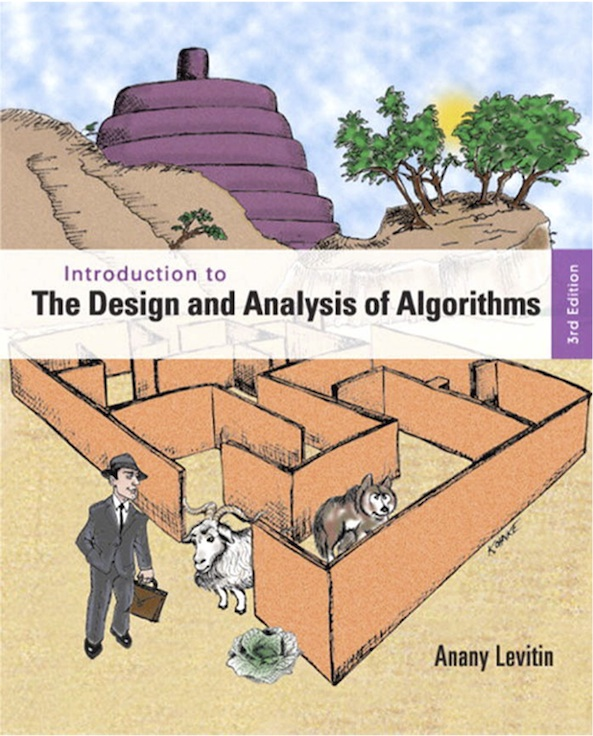
\includegraphics[height=.8\textheight]{img/capa-levitin.jpg}
  \end{center}
\end{frame}

\section{Considerações iniciais}

\begin{frame}
  \frametitle{Terminologia}

  \begin{itemize}
  \item eficácia temporal, complexidade temporal:
    \begin{itemize}
    \item quão rápido o algoritmo se executa? 
    \item quantos ciclos de processadores são necessários para executar o
      algoritmo?
    \end{itemize}
  \item eficácia espacial, complexidade espacial:
    \begin{itemize}
    \item quanta memória o algoritmo requer para armazenar os dados que manipula?
    \item quantas unidades de memória precisam ser alocadas?
    \end{itemize}
  \end{itemize}
\end{frame}

\begin{frame}
  \frametitle{Motivação}

  \begin{itemize}
  \item recursos computacionais escassos;
  \item computação móvel, computação ubíqua: computação = energia;
  \item geralmente a velocidade é um recurso mais crítico;
  \item tempo de execução tem sido o aspecto onde ganhos são maiores
  \end{itemize}
  \pause
  \alert{Foco na complexidade temporal}
\end{frame}

\section{Medição do tamanho da entrada}

\begin{frame}
\frametitle{Parâmetro da complexidade}

\begin{block}{Observação}
Para quase todos os algoritmos, quanto maior for o tamanho da entrada, maior
é o número de computações necessárias.
\end{block}

É natural querer definir a complexidade de um algoritmo em função do tamanho da
entrada.
\end{frame}

\begin{frame}
\frametitle{Exemplos}

\begin{itemize}
\item processamento de uma lista: o número de elementos na lista;
\item processamento de uma matriz: o número de linhas e colunas da matriz;
\item processamento em grafo: número de vértices, número de arestas;
\item processamento de números: número de bits usados para representar os
  números ($\lfloor \log_2 n \rfloor + 1$).
\item verificar se uma fórmula de lógica Booleana é válida: número de variáveis
  proposicionais.
\end{itemize}

\end{frame}

\begin{frame}
\frametitle{Exercícios}
\begin{enumerate}
\item calcular a soma de $n$ números;
\item calcular $n!$;
\item encontar o maior elemento em uma lista de $n$ elementos;
\item algoritmo para multiplicar dois inteiros decimais de $n$ dígitos cada;
\item crivo de Eratóstenes;
\item algoritmo de Euclides.
\end{enumerate}
\end{frame}

\section{Medição do tempo de execução}

\begin{frame}
  \frametitle{Unidade de medição do tempo de execução de um algoritmo}
    
  \begin{block}{Abordagem ingénua}
    \begin{itemize}
      \item implementar o algoritmo na sua linguagem de programação favorita;
      \item medir o tempo de execução da implementação para diferentes entradas é ingénua
      \end{itemize}
      Problemas:
      \begin{itemize}
      \item características do hardware tem influência;
      \item compilador tem influência;
      \item dificuldade de medição precisa.
      \end{itemize}
      \alert{Não é satisfatório}
    \end{block}
    
\end{frame}
\begin{frame}
  \frametitle{Unidade de medição do tempo de execução de um algoritmo}
    
  Precisamos de uma abordagem que não dependa de fator externos ao algoritmo.

  \begin{itemize}
  \item contar quantas vezes cada comando do algoritmo é executado.
  \end{itemize}

  Exemplo (Cormen et al.)
\end{frame}

\begin{frame}
  \frametitle{Exemplo}

    \begin{codebox}
    \Procname{$\proc{Insertion-Sort}(A)$}
    \li \For $j = 2$ \To $\id{length}[A]$ \> \> \> \> \> \> \> \> \> \> $c_1$ \> $n$
    \li \Do 
    \li   $\id{key} \gets A[j]$ \> \> \> \> \> \> \> \> $c_2$ \> $n-1$
    \li   $i \gets j-1$ \> \> \> \> \> \> \> \> $c_3$ \> $n-1$
    \li   \While $i > 0 \land A[i] > \id{key}$  \> \> \> \> \> \> \> \> $c_4$ \> $\sum_{j=2}^{n} t_j$
    \li   \Do
    \li     $A[i+1] \gets A[i]$ \> \> \> \> \> \> $c_5$ \> $\sum_{j=2}^{n} (t_j-1)$
    \li     $i \gets i - 1$     \> \> \> \> \> \> $c_6$ \> $\sum_{j=2}^{n} (t_j-1)$
          \End
    \li   $A[i+1] \gets \id{key}$ \> \> \> \> \> \> \> \> $c_7$ \> $n-1$
        \End
  \end{codebox}



  \begin{itemize}
  \item $c_i$: custo de executar cada linha
  \item $t_j$: número de vezes que o teste é efetuado para o elemento $A[j]$.
  \item custo total: $c_1.n+c_2.(n-1)+c_3.(n-1)+c_4.\sum_{j=2}^{n} t_j + c_5.\sum_{j=2}^{n} (t_j-1) + c_6.\sum_{j=2}^{n} (t_j-1)+c_7.(n-1)$
  \end{itemize}
\end{frame}

\begin{frame}
  \frametitle{Exemplo}

  $$
  \begin{array}{rcl}
    T(n) & = & \begin{array}[t]{l}
      c_1.n+c_2.(n-1)+c_3.(n-1)+c_4.\sum_{j=2}^{n} t_j + \\
      c_5.\sum_{j=2}^{n} (t_j-1) + c_6.\sum_{j=2}^{n} (t_j-1)+c_7.(n-1) \\
      \end{array} \\
    & = & (c_1+c_2+c_3+c_7).n  - (c_2 + c_3 + c_7) \\
    & & + c_4.\sum_{j=2}^{n} t_j+ (c_5+c_6).\sum_{j=2}^{n} (t_j-1)
  \end{array}
  $$

  Observamos que a complexidade do algoritmo depende de $n$, dos $t_i$ e dos
  $c_i$.
  \pause
  \begin{block}{Exercício}
    Os $c_i$ dependem da plataforma de execução, não de $A$.
    \begin{enumerate}
    \item Qual o menor valor possível para os $t_i$? Corresponde a qual situação?
    \item Qual o maior valor possível para os $t_i$? Corresponde a qual situação?
    \item Qual a complexidade do algoritmo nestas duas situações?
    \end{enumerate}
  \end{block}

\end{frame}

\begin{frame}

\frametitle{Exemplo: melhor caso}

    \begin{codebox}
    \Procname{$\proc{Insertion-Sort}(A)$}
    \li \For $j = 2$ \To $\id{length}[A]$ \> \> \> \> \> \> \> \> \> \> $c_1$ \> $n$
    \li \Do 
    \li   $\id{key} \gets A[j]$ \> \> \> \> \> \> \> \> $c_2$ \> $n-1$
    \li   $i \gets j-1$ \> \> \> \> \> \> \> \> $c_3$ \> $n-1$
    \li   \While $i > 0 \land A[i] > \id{key}$  \> \> \> \> \> \> \> \> $c_4$ \> $\sum_{j=2}^{n} t_j$
    \li   \Do
    \li     $A[i+1] \gets A[i]$ \> \> \> \> \> \> $c_5$ \> $\sum_{j=2}^{n} (t_j-1)$
    \li     $i \gets i - 1$     \> \> \> \> \> \> $c_6$ \> $\sum_{j=2}^{n} (t_j-1)$
          \End
    \li   $A[i+1] \gets \id{key}$ \> \> \> \> \> \> \> \> $c_7$ \> $n-1$
        \End
  \end{codebox}



  \begin{itemize}
    \item O teste do laço é avaliado uma vez apenas.
    \item $t_j = 1$ para $j = 2, \cdots n$
  \end{itemize}

\end{frame}

\begin{frame}

\frametitle{Exemplo: melhor caso}

$\sum_{j=2}^{n} 1 = n-1$ e $\sum_{j=2}^{n} 1 - 1 = 0$.

  $$
  \begin{array}{rcl}
    T(n) & = & (c_1+c_2+c_3+c_7).n  - (c_2 + c_3 + c_7) \\
    & & + c_4.\sum_{j=2}^{n} t_j+ (c_5+c_6).\sum_{j=2}^{n} (t_j-1) \pause \\
    & = & (c_1+c_2+c_3+c_7).n - (c_2 + c_3 +c_7) \\
    & & + c_4.(n-1) \pause \\
    \\
    T(n) & = & (c_1+c_2+c_3+c_4+c_7).n - (c_2 + c_3 + c_4 + c_7)
  \end{array}
  $$

\end{frame}

\begin{frame}

\frametitle{Exemplo: pior caso}

    \begin{codebox}
    \Procname{$\proc{Insertion-Sort}(A)$}
    \li \For $j = 2$ \To $\id{length}[A]$ \> \> \> \> \> \> \> \> \> \> $c_1$ \> $n$
    \li \Do 
    \li   $\id{key} \gets A[j]$ \> \> \> \> \> \> \> \> $c_2$ \> $n-1$
    \li   $i \gets j-1$ \> \> \> \> \> \> \> \> $c_3$ \> $n-1$
    \li   \While $i > 0 \land A[i] > \id{key}$  \> \> \> \> \> \> \> \> $c_4$ \> $\sum_{j=2}^{n} t_j$
    \li   \Do
    \li     $A[i+1] \gets A[i]$ \> \> \> \> \> \> $c_5$ \> $\sum_{j=2}^{n} (t_j-1)$
    \li     $i \gets i - 1$     \> \> \> \> \> \> $c_6$ \> $\sum_{j=2}^{n} (t_j-1)$
          \End
    \li   $A[i+1] \gets \id{key}$ \> \> \> \> \> \> \> \> $c_7$ \> $n-1$
        \End
  \end{codebox}



  \begin{itemize}
    \item O teste do laço é avaliado $j$ vezes.
    \item $t_j = j$ para $j = 2, \cdots n$
  \end{itemize}

\end{frame}

\begin{frame}

\frametitle{Exemplo: pior caso}

$\sum_{j=2}^{n} j = \frac{n(n+1)}{2} - 1.$
e
$\sum_{j=2}^{n} (j-1) = \frac{n(n-1)}{2}.$

  $$
  \begin{array}{rcl}
    T(n) & = & (c_1+c_2+c_3+c_7).n  - (c_2 + c_3 + c_7) \\
    & & + c_4.\sum_{j=2}^{n} t_j+ (c_5+c_6).\sum_{j=2}^{n} (t_j-1) \pause \\
    & = & (c_1+c_2+c_3+c_7).n - (c_2 + c_3 + c_7) \\
    & & c_4.(\frac{n(n+1)}{2} - 1) + (c_5+c_6).\frac{n(n-1)}{2} \pause \\
    \\
    T(n)
    & = & \frac{c_4+c_5+c_6}{2}.n² + \\
    & &   (c_1+c_2+c_3+\frac{c_4}{2}-\frac{c_5}{2}-\frac{c_6}{2} + c_7).n \\
    & & - (c_2 + c_3 + c_4 + \frac{c_5}{2} + \frac{c_6}{2} + c_7)
  \end{array}
  $$

\end{frame}

\begin{frame}
\frametitle{O conceito de operação básica}

\begin{itemize}
\item Esta forma de análise é demasiadamente detalhista;
\item Estes detalhes são inúteis, pois os $c_i$ são fatores externos ao
  algoritmo.
\item Ao invés disto, deve-se identificar a operação predominante na execução
  do algoritmo: a \emph{operação básica}.
\item A operação básica é aquela operação mais executada pelo algoritmo.
\item Basta contar quantas vezes o algoritmo executa a operação básica.
\end{itemize}
\begin{block}{Ponto chave}
O arcabouço clássico de análise de complexidade de algoritmos é contar quantas vezes a operação básica é executada, em função do tamanho da entrada $n$.
\end{block}
\end{frame}

\begin{frame}
\frametitle{Identificação da operação básica}

\begin{block}{Dica}
Em algoritmos iterativos, é a operação que fica no laço mais aninhado.
\end{block}

\pause

  \begin{codebox}
    \Procname{$\proc{Insertion-Sort}(A)$}
    \li \For $j = 2$ \To $\id{length}[A]$ \> \> \> \> \> \> \> \> \> \> $c_1$ \> $n$
    \li \Do 
    \li   $\id{key} \gets A[j]$ \> \> \> \> \> \> \> \> $c_2$ \> $n-1$
    \li   $i \gets j-1$ \> \> \> \> \> \> \> \> $c_3$ \> $n-1$
    \li   \While $i > 0 \land A[i] > \id{key}$  \> \> \> \> \> \> \> \> $c_4$ \> $\sum_{j=2}^{n} t_j$
    \li   \Do
    \li     $A[i+1] \gets A[i]$ \> \> \> \> \> \> $c_5$ \> $\sum_{j=2}^{n} (t_j-1)$
    \li     $i \gets i - 1$     \> \> \> \> \> \> $c_6$ \> $\sum_{j=2}^{n} (t_j-1)$
          \End
    \li   $A[i+1] \gets \id{key}$ \> \> \> \> \> \> \> \> $c_7$ \> $n-1$
        \End
  \end{codebox}



  Em outras palavras: quantas comparações são necessárias para ordenar uma
  sequência de $n$ elementos com o algoritmo de ordenação por inserção?

\end{frame}

\begin{frame}
  \frametitle{Exercício}

Qual a operação básica do algoritmo de busca linear?
\begin{codebox}
\Procname{$\proc{Linear-Search}(A, v)$}
\li $j \gets 1$
\li \While $A[j] \neq v$ and $j \le \id{length}(A)$
\li \Do
      $j \gets j+1$
    \End
\li \If $j \le \id{length}(A)$
\li \Then
      \Return $j$
\li \Else
      \Return \const{nil}
    \End
\end{codebox}  

\end{frame}

\begin{frame}
  \frametitle{Exercício}

  \begin{enumerate}
  \item Considere o algoritmo de soma de duas matrizes $N \times N$.
    Qual a operação básica? Quantas vezes é executada?
  \item Considere o algoritmo de multiplicação de duas matrizes $N \times N$.
    Qual a operação básica? Quantas vezes é executada?
  \end{enumerate}

\end{frame}

\begin{frame}
  \frametitle{Considerações}

  \begin{itemize}
  \item Considere um algoritmo qualquer.
  \item Seja $c$ o custo da execução da operação básica.
  \item Seja $C(n)$ o número de vezes que esta operação é executada pelo
    algoritmo.
  \item O tempo de execução do algoritmo $T(n)$, para uma entrada de tamanho $n$
    é tal que $T(n) \approx c \times C(n)$.
  \item Atenção $T(n)$ é \emph{aproximado}: 
    \begin{itemize}
      \item $c$ é aproximado, 
      \item as operações básicas não são contabilizadas.
      \item é uma estimativa razoável menos no caso de $n$ ser muito pequeno ou
        muito grande.
      \end{itemize}
  \end{itemize}

\end{frame}

\begin{frame}
  \frametitle{Perguntas}

  $$T(n) \approx c \times C(n).$$

  \begin{itemize}
  \item Quantas vezes mais rápido será executado o algoritmo em um computador 10
    vezes mais rápido?

    \only<2->{\alert{10}}
  \item Assumindo $C(n) = \frac{1}{2}.n.(n-1)$: quantas vezes mais lento será o
    algoritmo se multiplicamos o tamanho da entrada por dois?

    \only<3>{\begin{eqnarray*}
        T(2n)/T(n) & = & \frac{c \times C(2n)}{c \times C(n)} = \frac{C(2n)}{C(n)} \\
        & = & \frac{2n.(2n-1)}{n.(n-1)} = \frac{4n^2 - 2n}{n^2 - n} \\
        & \approx & 4 \mbox{ se $n$ for grande}
        \end{eqnarray*}}
  \end{itemize}

\end{frame}

\begin{frame}
  \frametitle{Observações}

  Para responder a pergunta:
  \begin{itemize}
  \item Assumindo $C(n) = \frac{1}{2}.n.(n-1)$: quantas vezes mais lento será o
    algoritmo se multiplicamos o tamanho da entrada por dois?
  \end{itemize}
  \pause
  Observe que:
  \begin{enumerate}
  \item Não precisamos saber o valor de $c$ para responder: ele foi
    simplificado.
  \item O fator multiplicativo $\frac{1}{2}$ também foi simplificado.
  \item Em $C(n)$ apenas o monômio de maior coeficiente foi determinante para
    calcular o resultado (assumindo $n$ é grande o suficiente).
  \end{enumerate}
  \begin{block}{Ponto chave}
    A análise de algoritmos desconsidera os fatores multiplicativos, e
    concentra-se no \emph{crescimento asintótico} considerando entradas de
    grande tamanho.
  \end{block}
\end{frame}

\section{Ordens de crescimento}

\begin{frame}
\frametitle{Crescimento asintótico}

\begin{itemize}
  \item O custo do algoritmo para entradas pequenas é geralmente irrelevante.
  \item A diferença entre algoritmos se faz com entradas de grande tamanho.
  \item Para entradas de grande tamanho, a crescimento asintótico do custo
    de computação é o aspecto mais importante.
\end{itemize}
\end{frame}

\begin{frame}
\frametitle{Valores (aproximados) de funções significativas}

$$
\begin{array}{c|ccccccc}
n & \log_2 n & n & n \log_2 n & n^2 & n^3 & 2^n & n! \\
\hline
\hline
10 & 3,3 & 10 & 3,3 \times 10^1 & 10^2 & 10^3 & 10^3 & 3,6\times 10^6 \\
10^2 & 6,6 & 10^2 & 6,6 \times 10^2 & 10^4 & 10^6 & 1,3 \times 10^{30} & 9,3\times 10^{157} \\
10^3 & 10 & 10^3 & 1,0 \times 10^4 & 10^6 & 10^9 &  &  \\
10^4 & 13 & 10^4 & 1,3 \times 10^5 & 10^6 & 10^9 &  &  \\
10^5 & 17 & 10^5 & 1,7 \times 10^6 & 10^{10} & 10^{15} &  &  \\
10^6 & 20 & 10^6 & 2,0 \times 10^7 & 10^{12} & 10^{18} &  & 
\end{array}
$$

\only<2>{A função logaritmo é a que cresce mais devagar. 
\begin{itemize}
\item Algoritmos de complexidade logarítmica tem custo imperceptível.
\item A base do logaritmo é irrelevante: $\log_a n = \log_b n \times \log_a b$.
  As funções só são diferentes por uma constante multiplicativa.
\end{itemize}
}

\only<3>{As funções $2^n$ e $n!$ tem crescimento muito rápido.
\begin{itemize}
\item Para qualquer entrada não pequena, o valor é astronômico;
\item O tempo de execução para entradas grandes excede a idade estimada
do universo.
\item Não são práticos para entradas que não sejam pequenas.
\end{itemize}
}

\end{frame}

\begin{frame}
\frametitle{Exercício}

Como reagem essas funções quando $n$ é duplicado? quadruplicado?

\begin{itemize}
\item $\log_2 n$
\item $n$
\item $n \log_2 n$
\item $n^2$
\item $n^3$
\item $2^n$
\item $n!$
\end{itemize}

\end{frame}

\begin{frame}
\frametitle{Exercício}

Para cada par de funções, indique se a primeira tem maior crescimento asintótico
que a segunda, menor crescimento asintótico, ou se os crescimentos asintóticos
são iguais:
\begin{itemize}
\item $n.(n+1)$ e $2000.n^2$;
\item $\log_2 n$ e $\ln n$;
\item $2^{n-1}$ e $2^n$;
\item $100.n^2$ e $0,01.n^3$;
\item $\log_2^2 n$ e $\log_2 n^2$;
\item $(n-1)!$ e $n!$.
\end{itemize}

\end{frame}

\section{Pior caso, melhor caso, caso médio, análise amortizada}

\begin{frame}
\frametitle{Pior caso, melhor caso, caso médio}

\begin{itemize}
\item A complexidade do algoritmo de \emph{ordenação por inserção} depende não
  só do tamanho da entrada, mas também do valor desta entrada.
\item A complexidade do algoritmo de \emph{busca linear} depende não só do
  tamanho da entrada, mas também do valor desta entrada.
\end{itemize}
\pause
\begin{description}
\item[pior caso] é a função que relaciona o tamanho da entrada $n$ ao maior tempo de execução possível para tratar uma entrada de tamanho $n$.
\item[melhor caso] é a função que relaciona o tamanho da entrada $n$ ao menor tempo de execução possível para tratar uma entrada de tamanho $n$.
\item[caso médio] é a função que relaciona o tamanho da entrada $n$ ao tempo médio de execução possível para tratar uma entrada de tamanho $n$, \emph{assumindo uma distribuição probabilística} das entradas possíveis.
\end{description}
\end{frame}

\section{Notação $\Theta$}

\begin{frame}

\frametitle{Exemplo: crescimento asintótico}

  $$
  \begin{array}{rcl}
    T(n)
    & = & \frac{c_4+c_5+c_6}{2}.n² + \\
    & &   (c_1+c_2+c_3+\frac{c_4}{2}-\frac{c_5}{2}-\frac{c_6}{2} + c_7).n \\
    & & - (c_2 + c_3 + c_4 + \frac{c_5}{2} + \frac{c_6}{2} + c_7) \\
    \\
    T(n) & = & a.n² + b.n + c \mbox{ onde $a, b, c$ são constantes que dependem da plataforma de execução.}
  \end{array}
  $$

  Quando $n$ é grande, o fator predominante é $a.n²$.

  Diz se que
  
  \begin{itemize}

    \item $T(n) \in \Theta(n²)$.

    \item O crescimento asintótico do tempo de execução é $n²$.

    \item O algoritmo é \emph{quadrático}.

  \end{itemize}
  
\end{frame}

\end{document}
